\documentclass[11pt]{article}
\usepackage[utf8]{inputenc}
\usepackage[T1]{fontenc}
\usepackage{amsmath}
\usepackage{amssymb}
\usepackage{multicol}
\usepackage{geometry}
\usepackage{tikz}
\usetikzlibrary{shapes,patterns,angles,quotes,calc,3d}
\usepackage{enumitem}
\usepackage{xcolor}
\usepackage{titlesec}

% Configurações de layout
\geometry{a4paper, left=1cm, right=1cm, top=0.5cm, bottom=1.2cm}
\setlength{\columnseprule}{0.4pt}

% Cores para títulos
\titleformat{\section}{\normalfont\Large\bfseries\color{blue}}{\thesection}{1em}{}
\titleformat{\subsection}{\normalfont\large\bfseries\color{red}}{\thesubsection}{1em}{}

\title{\textcolor{red}{Geometria Espacial
    \\Cálculo de Volume de Sólidos}}
\author{Professor: Jefferson}
\date{}

\begin{document}

\maketitle
\vspace{-1cm}

%\begin{center}
%\large{Nome: \underline{\hspace{8cm}} \quad Turma: \underline{\hspace{3cm}}}
%\end{center}

\begin{multicols}{2}

\section*{Conceito de Volume}

\textbf{Volume} é a medida do espaço ocupado por um sólido tridimensional, expressa em unidades cúbicas (m³, cm³, L, etc.).

\subsection*{Unidades de Medida}
\begin{itemize}
\item km³ (quilômetro cúbico)
\item m³ (metro cúbico)
\item dm³ (decímetro cúbico) = 1 litro
\item cm³ (centímetro cúbico) = 1 mL
\item mm³ (milímetro cúbico)
\end{itemize}

\subsection*{Conversões Importantes}
\begin{itemize}
\item 1 m³ = 1000 L
\item 1 dm³ = 1 L
\item 1 cm³ = 1 mL
\item 1 m³ = 1.000.000 cm³
\end{itemize}

\section*{Fórmulas Fundamentais}

\subsection*{Cubo}

\begin{center}
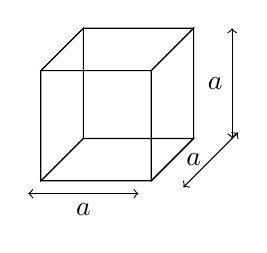
\begin{tikzpicture}[scale=0.7]
% Cubo em perspectiva
\begin{scope}[canvas is yz plane at x=0]
\draw (0,0) rectangle (2,2);
\end{scope}
\begin{scope}[canvas is xz plane at y=0]
\draw (0,0) rectangle (2,2);
\end{scope}
\begin{scope}[canvas is xy plane at z=0]
\draw (0,0) rectangle (2,2);
\end{scope}
\draw (2,0,0) -- (2,2,0) -- (2,2,2) -- (2,0,2) -- cycle;
\draw (0,2,0) -- (2,2,0) -- (2,2,2) -- (0,2,2) -- cycle;
\draw (0,0,2) -- (2,0,2) -- (2,2,2) -- (0,2,2) -- cycle;
% Medidas
\draw[<->] (-1,-1.0,0) -- (1,-1.0,0) node[midway,below] {$a$};
\draw[<->] (2.7,0,0) -- (2.7,2,0) node[midway,left] {$a$};
\draw[<->] (2.7,0,-0.28) -- (2.7,0,2.3) node[midway,left] {$a$};
\end{tikzpicture}
\end{center}

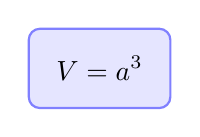
\begin{tikzpicture}
\node[rectangle, fill=blue!10, rounded corners, inner sep=10pt, draw=blue!50, thick] (box) {
$\displaystyle V = a^3$
};
\end{tikzpicture}

\textbf{Onde:}
\begin{itemize}
\item $a$ = medida da aresta
\end{itemize}

\subsection*{Paralelepípedo Retângulo}

\begin{center}
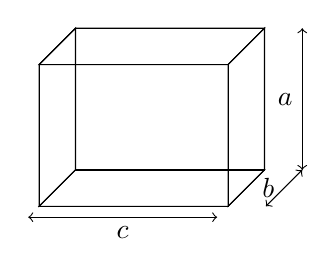
\begin{tikzpicture}[scale=0.6]
% Paralelepípedo
\begin{scope}[canvas is yz plane at x=0]
\draw (0,0) rectangle (3,2);
\end{scope}
\begin{scope}[canvas is xz plane at y=0]
\draw (0,0) rectangle (4,2);
\end{scope}
\begin{scope}[canvas is xy plane at z=0]
\draw (0,0) rectangle (4,3);
\end{scope}
\draw (4,0,0) -- (4,3,0) -- (4,3,2) -- (4,0,2) -- cycle;
\draw (0,3,0) -- (4,3,0) -- (4,3,2) -- (0,3,2) -- cycle;
\draw (0,0,2) -- (4,0,2) -- (4,3,2) -- (0,3,2) -- cycle;
% Medidas
\draw[<->] (-1,-1.0,0) -- (3,-1.0,0) node[midway,below] {$c$};
\draw[<->] (4.8,0,0) -- (4.8,3,0) node[midway,left] {$a$};
\draw[<->] (4.8,0,-0.0) -- (4.8,0,2.0) node[midway,left] {$b$};
\end{tikzpicture}
\end{center}

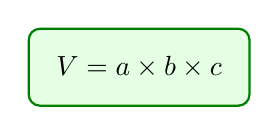
\begin{tikzpicture}
\node[rectangle, fill=green!10, rounded corners, inner sep=10pt, draw=green!50!black, thick] (box) {
$\displaystyle V = a \times b \times c$
};
\end{tikzpicture}

\textbf{Onde:}
\begin{itemize}
\item $a, b, c$ = comprimento, largura e altura
\end{itemize}

\subsection*{Prisma}

\begin{center}
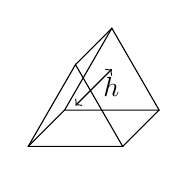
\begin{tikzpicture}[scale=0.6]
% Prisma triangular
\draw (0,0,0) -- (2,0,0) -- (1,1.732,0) -- cycle; % Base
\draw (0,0,2) -- (2,0,2) -- (1,1.732,2) -- cycle; % Topo
\draw (0,0,0) -- (0,0,2); % Arestas laterais
\draw (2,0,0) -- (2,0,2);
\draw (1,1.732,0) -- (1,1.732,2);
% Medidas
\draw[<->] (1,0.866,0) -- (1,0.866,2) node[midway,right] {$h$};
\end{tikzpicture}
\end{center}

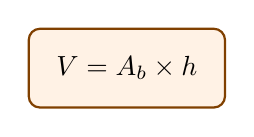
\begin{tikzpicture}
\node[rectangle, fill=orange!10, rounded corners, inner sep=10pt, draw=orange!50!black, thick] (box) {
$\displaystyle V = A_b \times h$
};
\end{tikzpicture}

\textbf{Onde:}
\begin{itemize}
\item $A_b$ = área da base
\item $h$ = altura
\end{itemize}

\subsection*{Cilindro}

\begin{center}
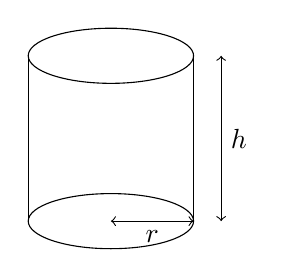
\begin{tikzpicture}[scale=0.7]
% Cilindro
\draw (0,0) ellipse (1.5 and 0.5); % Base inferior
\draw (-1.5,0) -- (-1.5,3); % Lado esquerdo
\draw (1.5,0) -- (1.5,3); % Lado direito
\draw (0,3) ellipse (1.5 and 0.5); % Base superior
% Medidas
\draw[<->] (0,0) -- (1.5,0) node[midway,below] {$r$};
\draw[<->] (2,0) -- (2,3) node[midway,right] {$h$};
\end{tikzpicture}
\end{center}

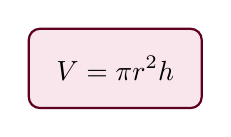
\begin{tikzpicture}
\node[rectangle, fill=purple!10, rounded corners, inner sep=10pt, draw=purple!50!black, thick] (box) {
$\displaystyle V = \pi r^2 h$
};
\end{tikzpicture}

\textbf{Onde:}
\begin{itemize}
\item $r$ = raio da base
\item $h$ = altura
\end{itemize}

\subsection*{Pirâmide}

\begin{center}
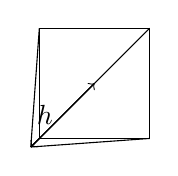
\begin{tikzpicture}[scale=0.7]
% Pirâmide quadrada
\draw (0,0,0) -- (2,0,0) -- (2,2,0) -- (0,2,0) -- cycle; % Base
\draw (1,1,0) -- (1,1,3); % Altura
\draw (0,0,0) -- (1,1,3); % Arestas laterais
\draw (2,0,0) -- (1,1,3);
\draw (2,2,0) -- (1,1,3);
\draw (0,2,0) -- (1,1,3);
% Medidas
\draw[<->] (1,1,0) -- (1,1,3) node[midway,left] {$h$};
\end{tikzpicture}
\end{center}

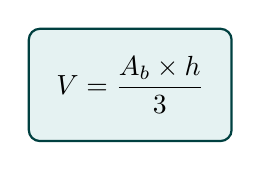
\begin{tikzpicture}
\node[rectangle, fill=teal!10, rounded corners, inner sep=10pt, draw=teal!50!black, thick] (box) {
$\displaystyle V = \frac{A_b \times h}{3}$
};
\end{tikzpicture}

\subsection*{Cone}

\begin{center}
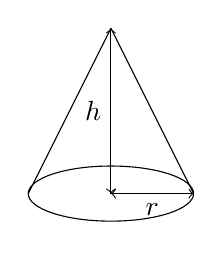
\begin{tikzpicture}[scale=0.7]
% Cone
\draw (0,0) ellipse (1.5 and 0.5); % Base
\draw (0,0) -- (0,3); % Altura
\draw (-1.5,0) -- (0,3); % Geratriz
\draw (1.5,0) -- (0,3); % Geratriz
% Medidas
\draw[<->] (0,0) -- (1.5,0) node[midway,below] {$r$};
\draw[<->] (0,0) -- (0,3) node[midway,left] {$h$};
\end{tikzpicture}
\end{center}

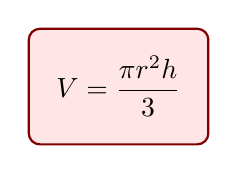
\begin{tikzpicture}
\node[rectangle, fill=red!10, rounded corners, inner sep=10pt, draw=red!50!black, thick] (box) {
$\displaystyle V = \frac{\pi r^2 h}{3}$
};
\end{tikzpicture}

\subsection*{Esfera}

\begin{center}
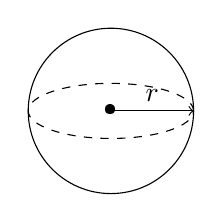
\begin{tikzpicture}[scale=0.7]
% Esfera
\draw (0,0) circle (1.5);
\draw[dashed] (0,0) ellipse (1.5 and 0.5);
% Raio
\draw[->] (0,0) -- (1.5,0) node[midway,above] {$r$};
\node at (0,0) {•};
\end{tikzpicture}
\end{center}

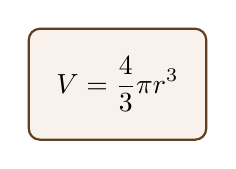
\begin{tikzpicture}
\node[rectangle, fill=brown!10, rounded corners, inner sep=10pt, draw=brown!50!black, thick] (box) {
$\displaystyle V = \frac{4}{3} \pi r^3$
};
\end{tikzpicture}

\section*{Exercícios Básicos}

\begin{enumerate}[leftmargin=*]

\item Calcule o volume dos sólidos:
\begin{enumerate}[label=\alph*)]
\item Cubo com aresta 4 cm
\item Paralelepípedo: 5 cm × 3 cm × 2 cm
\item Cilindro: $r = 7$ cm, $h = 10$ cm ($\pi \approx 3,14$)
\item Esfera: $r = 6$ cm
\end{enumerate}

\item Complete a tabela:

\begin{center}
\begin{tabular}{|c|c|c|c|}
\hline
\textbf{Sólido} & \textbf{Dados} & \textbf{Fórmula}   \\
\hline
Cubo & $a = 3$ m & $V = a^3$  \\
\hline
Paralelepípedo & $4 \times 5 \times 6$ cm & $V = a \times b \times c$  \\
\hline
Cilindro & $r = 2$ m, $h = 5$ m & $V = \pi r^2 h$  \\
\hline
Esfera & $r = 10$ cm & $V = \frac{4}{3} \pi r^3$  \\
\hline
\end{tabular}
\end{center}

\item Resolva os problemas:
\begin{enumerate}[label=\alph*)]
\item Uma caixa d'água cúbica tem 2 m de aresta. Quantos litros de água ela comporta?
\item Um tanque cilíndrico tem raio 1 m e altura 3 m. Qual seu volume em litros?
\item Uma esfera tem volume 36$\pi$ cm³. Qual seu raio?
\end{enumerate}

\item Conversão de unidades:
\begin{enumerate}[label=\alph*)]
\item 5 m³ = \underline{\hspace{1cm}} L
\item 2500 cm³ = \underline{\hspace{1cm}} L
\item 3,5 L = \underline{\hspace{1cm}} cm³
\end{enumerate}

\section*{Exercícios Intermediários}

\begin{enumerate}[leftmargin=*, start=5]

\item Prisma triangular:
\begin{enumerate}[label=\alph*)]
\item Base: triângulo retângulo com catetos 3 cm e 4 cm
\item Altura do prisma: 10 cm
\item Calcule o volume
\end{enumerate}

\item Pirâmide de base quadrada:
\begin{enumerate}[label=\alph*)]
\item Lado da base: 6 cm
\item Altura da pirâmide: 8 cm
\item Calcule o volume
\end{enumerate}

\item Cone:
\begin{enumerate}[label=\alph*)]
\item Raio da base: 5 cm
\item Altura: 12 cm
\item Calcule o volume
\end{enumerate}

\item Comparação de volumes:
\begin{enumerate}[label=\alph*)]
\item Cubo de aresta 4 cm vs Esfera de raio 3 cm
\item Cilindro: $r = 2$ cm, $h = 5$ cm vs Cone: $r = 3$ cm, $h = 4$ cm
\end{enumerate}

\item Problemas contextualizados:
\begin{enumerate}[label=\alph*)]
\item Uma piscina retangular mede 8 m × 4 m × 1,5 m. Quantos litros de água são necessários para enchê-la?
\item Uma lata de refrigerante cilíndrica tem 6,5 cm de diâmetro e 12 cm de altura. Qual seu volume em mL?
\item Quantas bolinhas de gude (esferas de raio 1 cm) cabem em uma caixa cúbica de 10 cm de aresta?
\end{enumerate}

\item Sólidos semelhantes:
\begin{enumerate}[label=\alph*)]
\item Dois cubos são semelhantes com razão 1:3. Qual a razão entre seus volumes?
\item Um cone tem volume 27 cm³. Qual o volume de um cone semelhante com o dobro das dimensões lineares?
\end{enumerate}

\end{enumerate}

\section*{Exercícios Avançados}

\begin{enumerate}[leftmargin=*, start=11]

\item Demonstre as fórmulas:
\begin{enumerate}[label=\alph*)]
\item Demonstre que $V = a^3$ para o cubo
\item Deduza $V = \dfrac{4}{3} \pi r^3$ para a esfera
\item Mostre que $V = \dfrac{A_b \times h}{3}$ para pirâmides
\end{enumerate}

\item Relação entre volumes:
\begin{enumerate}[label=\alph*)]
\item Mostre que o volume de uma esfera é $\frac{2}{3}$ do volume do cilindro circunscrito
\item Prove que o volume de um cone é $\frac{1}{3}$ do volume do cilindro de mesma base e altura
\end{enumerate}

\item Volume por integração:
\begin{enumerate}[label=\alph*)]
\item Calcule o volume da esfera usando integração
\item Encontre o volume de um cone por integração
\end{enumerate}

\item Sólidos de revolução:
\begin{enumerate}[label=\alph*)]
\item Qual sólido obtemos ao girar um triângulo retângulo em torno de um cateto?
\item Calcule o volume do sólido obtido girando $y = x^2$ de 0 a 1 em torno do eixo x
\end{enumerate}

\item Volume de troncos:
\begin{enumerate}[label=\alph*)]
\item Tronco de pirâmide: $V = \frac{h}{3}(A_1 + A_2 + \sqrt{A_1 A_2})$
\item Tronco de cone: $V = \frac{\pi h}{3}(R^2 + Rr + r^2)$
\end{enumerate}

\item Problema histórico:
\begin{enumerate}[label=\alph*)]
\item Como Arquimedes descobriu a fórmula da esfera?
\item Explique o método de exaustão para volumes
\end{enumerate}

\item Máximos e mínimos:
\begin{enumerate}[label=\alph*)]
\item De todos os cilindros inscritos em uma esfera de raio R, qual tem maior volume?
\item Qual o paralelepípedo de maior volume com superfície total fixa?
\end{enumerate}

\item Volume de sólidos irregulares:
\begin{enumerate}[label=\alph*)]
\item Explique o princípio de Cavalieri
\item Como calcular o volume de uma pedra irregular?
\end{enumerate}

\item Aplicações práticas:
\begin{enumerate}[label=\alph*)]
\item Cálculo de dose de medicamento por volume corporal
\item Volume de concreto para uma laje
\item Capacidade de um silo agrícola
\end{enumerate}

\item Desafio final:
\begin{enumerate}[label=\alph*)]
\item Um cilindro e uma esfera têm mesmo volume e mesma altura. Qual a relação entre seus raios?
\item Qual sólido tem maior volume: cubo de aresta 2R ou esfera de raio R?
\end{enumerate}

\end{enumerate}

\section*{Resumo das Fórmulas}

\subsection*{Poliedros:}
\begin{itemize}
\item Cubo: $V = a^3$
\item Paralelepípedo: $V = a \times b \times c$
\item Prisma: $V = A_b \times h$
\item Pirâmide: $V = \dfrac{A_b \times h}{3}$
\end{itemize}

\subsection*{Corpos Redondos:}
\begin{itemize}
\item Cilindro: $V = \pi r^2 h$
\item Cone: $V = \dfrac{\pi r^2 h}{3}$
\item Esfera: $V = \dfrac{4}{3} \pi r^3$
\end{itemize}

\subsection*{Relações Importantes:}
\begin{itemize}
\item 1 m³ = 1000 L
\item 1 dm³ = 1 L
\item 1 cm³ = 1 mL
\item Volume de sólidos semelhantes: $V_1:V_2 = k^3$
\end{itemize}

\section*{Dicas para Cálculo}

\begin{itemize}
\item \textbf{Identifique o sólido}: Qual fórmula usar?
\item \textbf{Verifique unidades}: Todas na mesma unidade
\item \textbf{Use $\pi$ adequadamente}: 3,14 para aproximações, $\pi$ para exato
\item \textbf{Calcule área da base primeiro}: Para prismas e pirâmides
\item \textbf{Desenhe a figura}: Ajuda na visualização
\item \textbf{Faça estimativas}: Verifique se resultado é razoável
\end{itemize}

\section*{Aplicações Práticas}

\begin{itemize}
\item \textbf{Engenharia civil}: Volume de concreto
\item \textbf{Química}: Volume de reações
\item \textbf{Medicina}: Dosagem de medicamentos
\item \textbf{Logística}: Capacidade de contêineres
\item \textbf{Agricultura}: Volume de silos e reservatórios
\item \textbf{Indústria}: Capacidade de tanques e recipientes
\end{itemize}

\end{multicols}

\end{document}
